\documentclass[
  biblatex,
  seconds=true,
  language=slovak,
  figures=false,
  urldate=iso,
  glossaries,
  index
]{kidiplom}

\title{Paralelní Programování v Go}
\title[english]{Paralel programing in Go}

\author{Richard Bebjak}

\supervisor{Mgr. Jan Laštovička, Ph.D.}

\annotation{}

\annotation[english]{}

\keywords{}
\keywords[english]{}

\thanks{Děkuji, děkuji, děkuji.}

\bibliography{}

\usepackage{lipsum}
\usepackage{longtable}
\usepackage{listings}
\usepackage{biblatex}
\usepackage{graphicx}
\addbibresource{bebjak.bib}

\begin{document}
\maketitle

\newcommand{\BibLaTeX}{\textsc{Bib}\LaTeX}

\section{Čo je to Communication Sequential Process}
\textit{Communication Sequential Process} (CSP) je základný teoretický prístup ku súbežnému programovaniu.\cite{hoare1978}
Tento prístup definuje ako môžu súbežne bežiace procesy spolupracovať a komunikovať. Na rozdiel od tradičných prístupov založených
na zdiaľanej pamäti, CSP je založené na komunikácii medzi procesmi ako hlavným mechanizmom koordinácie. Procesy si neposkytujú priamy
prístup k pamäti, čím sa znižuje počet chýb súbehu. Základnou myšlienkou CSP je, že program sa skladá z viacerých sekvenčných procesov
vykonávaných súbežne, ktoré medzi sebou komunikujú prostredníctvom vstupno-výstupných operácií.

\subsection{Základné myšlienky CSP}
Hoare navrhol riešenie na základe troch princípov:
\begin{itemize}
	\item Strážené príkazy
	\item Paralelná kompozícia procesov
	\item Komunikácia pomocou vstupu a výstupu
\end{itemize}
Koncept strážených príkazov zavedený Djikstrom umožňuje riadiť vetvenie a nedeterministické správanie. Ide o príkazy, ktoré
sa vykonajú až po splnení určitej podmienky.
Paralelná kompozícia opisuje
program tak, že program môže pozostávať z viacerých procesov, ktoré sa spúšťajú súčasne, vykonávajú sa nezávisle a končia
až keď skončia všetky súbežné procesy. Komunikácia pomocou vstupu a výstupu znamená, že procesy spolu komunikujú výhradne
pomocou vstupno-výstupných operácií. Procesy tak nezdieľajú pamäť a ich komunikácia prebieha synchronizovane.

V CSP možno chápať každý proces ako samostatnú výpočtovú jednotku s vlastným stavom, ktorá vykonáva príkazy v definovanom poradí.
Procesy nie sú izolované, ich spolupráca je kľúčová na dosiahnutie požadovaného výsledku. Ich spolupráca je realizovaná
pomocou synchrónnej komunikácie, pri ktorej musí byť odosieľateľ aj prijímateľ pripravený na výmenu údajov v rovnakom okamihu.
Tento prístup eliminuje problémy spojené s chybami súbehu a nekonzistentným stavom pamäte. Tento prístp ale môže viesť k
situácii, kedy procesy čakajú bez možnosti pokračovať.

\subsection{Komunikácia v CSP}
Hlavnou vlastnosťou CSP je prenos dát medzi procesmi. Hodnota odoslaná jedným procesom je priamo priradená premennej v druhom
procese. Procesy musia byť pripravené na komunikáciu v rovnakom okamihu.
Prenos hodnoty je atomický a synchronizovaný, teda nemôže prísť k čiastočnému prenosu alebo nekonzistentnému stavu.
Zjednodušuje uvažovanie o správnosti programu, pretože eliminuje potrebu zamykania a konflikty pri prístupe k pamäti.
Kladú sa ale väčšie nároky na synchronizáciu procesov.

CSP používa príkazy:
\begin{itemize}
	\item Priradenie hodnoty
	\item Vstup
	\item Výstup
	\item Prázdny príkaz
	\item Štruktúrovaný príkaz
	      \begin{itemize}
		      \item Alternatívny príkaz
		      \item Repetitívny príkaz
	      \end{itemize}
\end{itemize}
Priradenie hodnoty premennej funguje ako ho poznáme. Vstup a výstup sú synchronizované tak, že proces posielajúci výstupnú operáciu musí
čakať kým proces s adekvátnou vstuponou operáciou je pripravený na komunikáciu a naopak. Štruktúrové príkazy umožňujú vytvárať
alternatívy a repetetívy. Alternatívny príkaz umožňuje výber z viacerých možností, podľa splnenia podmienky. Umožňuje
synchronizovanie medzi viacerými procesmi naraz. Podľa splnenia podmienky, ak nie je splnená žiadna podmienka, čaká. Ak je splnená
jedna podmienka vykoná proces priradený danej podmienke. Ak je splnených viacero podmienok, vykoná náhodnú, výber je
nedeterministický. Tento príkaz umožňuje modelovať situácie, kde správanie programu závisí od aktuálnych podmienok alebo
interakcie s inými procesmi. Repetitívny príkaz predstavuje cyklus alternatívnych príkazov, kedy sa príkaz vykonáva opakovane, kým je
splnená aspoň jedna podmienka. Inak sa cyklus ukončí. Tento príkaz umožňuje modelovať situácie, kde program reaguje na
prichádzajúce správy alebo udalosti.

\subsection{Výrobca a spotrebiteľ CSP}
CSP sa dá v tomto príklade chápať ako monitor s ktorým komunikujú viaceré procesy. Procesy musia byt odlišne pomenované napr. \uv{Výrobca} a \uv{Spotrebiteľ},
alebo odlišný index napríklad \uv{X(0)}. Každá komunikácia musí mať jednoznačne určený svoj zdroj alebo cieľ. Keď je monitor pripravený komunikovať
s ktorýmkoľvek používateľským procesom, zväčša ktorý príde prvý, používa strážený príkaz s rozsahom.
\[
	[(i:1..100);\; X(i)?(value\ parameters) \rightarrow \dots ;\; X(i)!(results);]
\]
Premenná \uv{i} sa poúžíva na posielanie výsledkov späť procesu, ktorý komunikáciu inicioval.

Ako monitor nie je pripravený na komunikáciu od konkrétneho procesu napríklad \uv{X(j)}, môže byť vstupný príkaz doplnený o booleovskú podmienku,
takzvanú stráž. Napríklad dve po sebe idúce požiadavky od rovnakého procesu, môžu byť zablokované pomocou podmienky \uv{j=0}.
\[
	*[(i:1..100)i\neq j;\; X(i)?(parameters) \rightarrow \dots ;\; i := j ;\;]
\]
V tomto prípade bude výstup procesu \uv{X(j)} odložený, kým nebude spracovaná požiadavka iného procesu.
Podobne je možné použiť podmienky na oddialenie prijatia vstupov, ktoré by porušili plánovacie obmedzenia. \cite{hoare1978}

\section{Goroutine}
Goroutine je funkcia ktorá sa vykonáva súbežne.
Nie sú to vlákna operačného systému ani vlákna riadené runtime prostredím. Ide o
vyššiu abstrakciu nazývanú korutiny v jazyku Go goroutine. Goroutines sú súbežné podprogramy, ktoré nemôžu byť
prerušené zvonka. Obsahujú však body, v ktorých môžu byť pozastavené a znovu spustené.
Na rozdiel od vláken je prepínanie medzi goroutine rýchlejšie približne o 1,242 $\mu\text{s}$.\cite{cox2017}
Goroutine sa dajú spustiť pomocou kľúčového slova \texttt{go}.
\begin{lstlisting}[language=Go]
	func main{
		go SayHello()
	}

	func SayHello(){
		fmt.Println("Hello")
	}
\end{lstlisting}
Je možné goroutine implementovať ako anonymné funkcie.
\begin{lstlisting}[language=Go]
	go func(){
		fmt.Println("Hello")
	}
\end{lstlisting}
Ako anonymné funkcie musia byť zavolané okamžite. Vieme goroutine priradiť do premennej.
\begin{lstlisting}[language=Go]
	sayHello := func(){
		fmt.Println("Hello")
	}

	go sayHello()
\end{lstlisting}
Goroutine sú špefické pre jazyk Go, pretože sú integrované do runtime prostredia Go.
Goroutine si sami neurčujú body pozastavenia. Runtime Go sleduje ich správanie a
automaticky ich pozastaví, a znovu spustí, keď sú opätovne pripravené pokračovať.
Goroutine bežia súbežne, čo nie je ich vlastnosťou, preto potrebujú mechanizmus, ktorý im umožní bežať a vykonávať sa
súbežne.

\subsection{Model a plánovač goroutine}
Go používa plánovač \uv{M:N} a model súbežnosti fork-join.\cite{cox2017}
Teda na \uv{M} vláknach sa vykonáva \uv{N} goroutine. Goroutine
sú mapované na tieto vlákna a go runtime sa stará o ich rozdelenie a efektívne vykonávanie. Stará sa o ich spúštanie,
ak je nejaká goroutine blokovaná tak go runtime môže spustiť inú.

Podľa modelu fork-join, \uv{Fork} znamená, že program môže vytvoriť novú
goroutine, ktorá sa vykonáva súbežne s rodičovským kódom. A \uv{Join} znamená, že sa tieto vetvy spoja v mieste nazývanom
join point.
\ref{fork-join}
Spájanie vetviev nie je funkciou programu, preto je nutná synchronizácia pri goroutine.


\section{Komunikačné kanály}
Komunikačné kanály predstavujú jeden zo základných mechanizmov synchronizácie a komunikácie medzi goroutines. Sú zabudované referečným typom,
ktorý umožňuje bezpečný prenos dát. Ich návrh vychádza z Communicating Sequential Processes,
ktorý zdôrazňuje komunikáciu medzi procesmi miesto zdieľania pamäte.\cite{cox2017}

Komunikačné kanály sa deklarujú pomocou kľúčového slova \texttt{chan}
a vždy sa deklarujú aj s určitým typom. To znamená, že kanál môže prenášať hodnoty
iba tohto typu.
Komunikačné kanály patria k referenčným typom, preto ich deklarácia nevytvára potrebnú pamäťovú štruktúru.
Pamäť sa alokuje pomocou zabudovanej funkcie \texttt{make}.
\begin{lstlisting}[language=Go]
    make(chan type, buffer_size)
\end{lstlisting}
Takto vytvorený komunikačný kanál umožňuje zapisovanie a čítanie hodnôt.
Zápis do komunikačného kanála umožnuje operátor \texttt{<-}, ktorý sa umiestňuje na pravú stranu názvu komunikačného kanála,
pre čítanie sa operátor umiestňuje na ľavú stranu názvu komunikačného kanála.
\begin{lstlisting}[language=Go]
    channel <- data
    variable = <- channel
\end{lstlisting}

Dôležitou vlastnosťou komunikačného kanála je jeho blokujúce správanie. Ak goroutine zapisuje do komnikačného kanála, ktorý je plný, je jej proces
blokovaný kým iná goroutine z komunikačného kanála hodnotu neprečíta. Podobne čítanie z prázdneho komunikačného kanála je blokované kým nie je do
komunikačného kanála zapísaná nová hodnota.

Komunikačný kanál je možné zavrieť pomocou funkcie \texttt{close}.
Pri čítaní z kanála je možné získať druhú návratovú hodnotu typu bool, ktorá indikuje jeho otvorenie.
Uzavretie teda signalizuje prijímateľovi, že do komunikačného kanála nebude viac zapisované. Ak odosielateľ pošle dáta do
uzavretého komunikačného kanálu,
program vráti error \texttt{panic: send on closed channel}. Po uzavretí komunikačného kanálu, prijímateľ nečaká na hodnotu
ale obdrží prázdnu hodnotu a hodnotu \uv{False} z druhej návratovej hodnoty.
Nasledujúci príklad demonštruje použitie.
\begin{lstlisting}[language=Go, numbers=left]
    var channel = make(chan int, 1)

    go func(){
        channel <- 42
    }()

    result := <- channel
    close(channel)
\end{lstlisting}
Na riadku jedna si vytvoríme komunikačný kanál s referečným typom int a veľkosťou buffera jedna. Na riadku tri spustíme novú goroutine.
Na riadku štyri v goroutine uložíme do komunikačného kanála hodnotu 42. Na riadku sedem hlavné vlákno čaká na dáta z komunikačného kanála. Ak dáta prídu,
uloží do premennej \uv{result} dáta z komunikačného kanála, v tomto prípade 42. Na riadku osem uzavrieme komunikačný kanál.

\subsection{Druhy komunikačných kanálov}
Každý komunikačný kanál môže byť bufferovaný alebo nebufferovaný. Nebufferovaný komunikačný kanál nemá žiadnu kapacitu a každá operácia zápisu musí
byť okamžite spravovaná operáciou čítania.

Bufferovaný komunikačný kanál sa definuje pomocou voliteľného druhého argumentu funkcie make.
Bufferovaný komunikačný kanál obsahuje buffer s definovanou kapacitou, ktorá umožní uložiť určitý počet hodnôt do buffera bez okamžitého čítania.
Bufferovaný komunikačný kanál zablokuje zápis až v momente keď je buffer plný.

Jazyk Go umožňuje definovanie jednosmerných kanálov, ktoré podporujú iba zápis alebo čítanie. Tieto komunikačné kanály sa používajú ako parametre
funkcií, aby určili akým spôsobom sa komunikačný kanál v danej časti programu používa. Tento mechanizmus zvyšuje bezpečnosť programu, pretože
kompilátor dokáže zachytiť nesprávne použitie.

\subsection{Implementácia}
V runtime prostredí je komunikačný kanál implementavaný ako štruktúra hchan. Obsahuje počet hodnôt v kanáli, maximálnu
kapacitu, ukazovateľ na buffer, fronty čakajúcich goroutine a synchronizačný zámok. Zjednodušene štruktúra obsahuje:
\begin{tabular}{p{4cm} p{10cm}}
	qcount uint        & Počet prvkov v bufferi                                            \\
	dataqsiz uint      & Veľkosť jednej hodnoty na bufferi                                 \\
	buf unsafe.Pointer & Pointer na buffer                                                 \\
	sendx uint         & Index pre zápis                                                   \\
	recvx uint         & Index pre čítanie                                                 \\
	recvq waitq        & Čakajúci prijímatelia                                             \\
	sendq waitq        & Čakajúci odosielatelia                                            \\
	closed uint32      & Hodnota určujúca či je komunikačný kanál otvorený alebo zatvorený \\
	lock mutex         & Mutex na prístup k bufferu                                        \\
\end{tabular}
Táto štruktúra ukazuje, že komunikačný kanál funguje ako kruhový buffer, doplnený o mechanizmi blokujúce goroutine.\cite{goChan}
Implementácia front \uv{sendq} a \uv{recvq} je hlavný prvok na synchronizáciu goroutine. Kedy odosielateľ čaká na príjemcu
a príjemca čaká na odosielateľa. To zabezpečuje bezpečnú synchronizáciu a absenciu problému súbehu zámkov v aplikačnom kóde.

Komunikačný kanál má operácie prijímanie a odosielanie hodnoty. Komunikačný kanál odosiela a prijíma dve hodnoty. Posielanú
hodnotu a hodnotu typu bool, ktorá značí, či je kanál otvorený.
Odosielanie hodnoty je implementované funkciou \texttt{chansend}.
Jej správanie závisí od aktuálneho stavu komunikačného kanála. Zjednodušene, rozlišuje tri stavy.
Ak existuje čakajúci príjemca, teda
je hodnota v recvq goroutine, hodnota sa prenesie priamo bez použitia bufferu.
\begin{lstlisting}[language=Go]
if receiver exist:
	copy data directly to receiver
	wake up receiver 	
\end{lstlisting}
Najrýchlejší scenár, nakoľko sa neukladá hodnota do bufferu. Ďalší stav, ak neexistuje čakajúci príjemca ale existuje voľné
miesto v bufferi. Tak sa hodnota uloží na buffer a zvýší sa počítadlo.
\begin{lstlisting}[language=Go]
if buffer not full:
	store value in buffer 
	increment qcount	
\end{lstlisting}
Tretí stav ak neexistuje čakajúci príjemca a neexistuje voľné miesto na bufferi. V takom prípade sa goroutine uloží do fronty
\uv{sendq} a čaká na uvoľnenie miesta na bufferi.

Prijímanie hodnoty je implementované funkciou \texttt{chanrecv}. Rovnako jej správanie závisí od aktuálneho stavu komunikačného
kanála. Zjednodušene rozlišuje tri stavy. Ak existuje čakajúci odosielateľ, teda je hodnota v sendq, hodnota sa prenesie priamo
bez použitia bufferu.
\begin{lstlisting}[language=Go]
if sender exist:
	receive value directly
	wake sender
\end{lstlisting}
Ak neexistuje čakajúci odosielateľ ale buffer obsahuje aspň jednu hodnotu, je táto hodnota načítaná a zníži sa hodnota počítadla.
\begin{lstlisting}[language=Go]
if buffer not empty:
	read value from buffer
	decrement qcount	
\end{lstlisting}
Ak neexistuje čakajúci odosielateľ a buffer neobsahuje žiadnu hodnotu. V takom prípade sa goroutine uloží do fronty \uv{recvq}
a čaká na odosielateľa.

Operácia uzavretia komunikačného kanála nastaví \uv{closed} na hodnotu \uv{False}. Zároveň sa odblokujú všetky čakajúce goroutine
v \uv{recvq}. Goroutine v prvej návratovej hodnote obdržia prázdnu hodnotu, čo nie je vždy chcené a je potrebná reakcia
programu na druhú návratovú hodnotu. Pri odosielaní na uzavretý komunikačný kanál, program vráti chybu.


\section{Synchronizačné primitíva}
Jazyk Go poskytuje sync balík, ktorý obsahuje synchronizačné primitíva. Tieto synchronizačné primitíva sú používané pri nízkoúrovňovom
prístupe do pamäte. Rozdiel medzi ostatnými jazykmi a jazykom Go je, že Go poskytuje novú sadu synchronizačných primitív pre súbežnosť nad sadou primitív pre synchronizáciu prístupu k pamäti.

\subsection{WaitGroup}
Je to nástroj z balíka sync, ktorého účelom je umožniť programu počkať na dokončenie skupiny goroutine pred tým, než bude pokračovať.
Mechanizmus sa využíva v prípade, že sa vykonáva viacero nezávislých úloh.
WaitGroup si môžeme predstaviť ako bezpečný čítač. Tento čítač eviduje počet goroutine, ktoré ešte nedokončili svoju činnosť.
Čítač sa zvyšuje pomocou metódy \texttt{Add(n)}, kde \uv{n} udáva počet goroutine, ktoré sa majú vykonať.
Čítač sa znižuje pomocou metódy \texttt{Done()}.
Program je zablokovaný na metóde \texttt{Wait()}, kým hodnota čítača nedosiahne nulovú hodnotu. Nasledujúci príklad demonštruje použitie.
\begin{lstlisting}[language=Go, numbers=left]
    var wg sync.WaitGroup

	for i := 0; i < 10; i++ {
		wg.Add(1)
		go func(i int) {
			defer wg.Done()
			fmt.Println("Goroutine", i)
			time.Sleep(200)
		}(i)
	}
	wg.Wait()
	fmt.Println("End")
\end{lstlisting}
Na prvom riadku si definujeme WaitGroup. Následne v cykle na riadku tri zvýšime hodnotu WaitGroup o jedna. Na riadku štyri pustíme novú goroutine.
V goroutine na riadku päť zabezpečíme, že po dokončení činnosti, zníži hodnotu WaitGroup o jedna.
Následne vykoná vypís a čakanie pre simuláciu paralelného výpočtu.
Na riadku jedenásť program čaká, kým hodnota WaitGroup bude nulová. následne vypíše \uv{End}.

\subsection{Mutex a RWMutex}
Mutex je nástroj z balíka sync, ktorého účelom je chrániť časť programu so zdieľanými zdrojmi, ku ktorým môže pristupovať iba jedna goroutine.
Pred vstupom do časti programu so zdieľanými zdrojmi, musí goroutine získať zámok pomocou metódy \texttt{Lock()}. Po ukončení činnosti
v danej časti programu, uvoľní zámok pomocou metódy \texttt{Unlock}. Počas držania zámku, nemôže iná goroutine vstúpiť do tejto časti programu.
RWMutex rozširuje Mutex o zámok, ktorý rozlišuje operácie čítania a zápisu. Metódy na získanie zámku \texttt{RLock() / Lock()},
metódy na uvoľnenie zámku \texttt{RUnlock() / Unlock()}. RWMutex umožňuje získať zámok pre čítanie viacerým goroutine,
ale pre zápis umožňuje získať zámok jednej goroutine. Počas zápisu nie je umožnené získať zámok pre čítanie. Pri zápise čaká kým sú uvoľnené
všetky zámky. Nasledujúci príklad demonštruje použitie.
\begin{lstlisting}[language=Go, numbers=left]
    var wg sync.WaitGroup
	var rw sync.RWMutex

	observer := func(i int) {
		defer wg.Done()
		rw.RLock()
		fmt.Println("Reading started", i)
		time.Sleep(400 * time.Millisecond)
		fmt.Println("Reading ends", i)
		rw.RUnlock()
	}

	writter := func(i int) {
		defer wg.Done()
		defer rw.Unlock()
		rw.Lock()
		fmt.Println("Writting started", i)
		time.Sleep(400 * time.Millisecond)
		fmt.Println("Writting ended", i)
	}

	for i := 0; i < 100; i++ {
		wg.Add(1)
		if i%25 == 0 {
			go writter(i)
		} else {
			go observer(i)
		}
	}
	wg.Wait()
	fmt.Println("End")
    
\end{lstlisting}
Na riadku dva si definujeme RWMutex. Na riakdu štyri si definujeme funkciu čitateľa, ktorá sa pokúsi získať zámok pre čítanie
vypíše, že začala, počká, vypíše, že skončila a po skončení uvoľní zámok pre čítanie.
Na riadku trinásť si definujeme funkciu zapisovateľa, ktorá sa pokúsi získať zámok, vypíše, že začala, počká, vypíše, že skončila
a po skončení uvoľní zámok.
Na riadku dvadsaťdva je cyklus, v ktorom voláme funkciu zapisovateľa ak \uv{i} modulo 25 je nula, inak voláme funkciu čitateľa.
Následne počkáme na dokončenie všetkých goroutine a vypíšeme, že sme skončili. Výsledok tohto kódu bude približne.
\begin{lstlisting}
    "Writting started 0"
    "Writting ended 0"
    "Reading started 1"
    "Reading started 2"
    "Reading started 5"
    ...
    "Reading ended 98"
    "Reading ended 97"
    "Reading ended 99"
    "Writting started 50"
    "Writting ended 50"
    "Writting started 75"
    "Writting ended 75"
\end{lstlisting}
Z tohto výsledku vidíme, že RWMutex uprednostňuje čitateľov. Vynútenie zámku pre zapisovateľa je možné pomocou ďalších
synchronizačných nástrojov, ako napríklad pomocou komunikačných kanálov.


\newpage
\section{Select}
\section{Chat server}
Navrhnutý prototyp serveru je založený na architektúre klient-server, kde server zabezpečuje výmenu správ medzi pripojenými
klientmi. Komunikácia medzi klientom a serverom je realizovaná cez Transmission Control Protocol (TCP), ktorý zabezpečuje
spoľahlivý prenos dát, zachovanie poradia správ a detekciu chýb pri prenose. Server je implementovaný v programovacom jazyku Go,
využívajúc jeho vstavanú podporu pre súbežné programovanie prostredníctvom goroutine. Hlavná úloha servera spočíva v prijímaní
nových klientskych spojení, spracovaní ich požiadavkov a správe komunikačných miestností.

\subsection{Klientské spojenie}
\begin{lstlisting}[language=Go]
	for{
		conn, err := ln.Accept()
		go clientHandle.HandleConnection(conn)
	}
\end{lstlisting}

Pri spustení server vytvorí TCP listener \uv{ln}. Následne v nekonečnom cykle
čaká na nové pripojenie, ak je pripojenie úspešné tak vytvorí pre to spojenie novú goroutine. Týmto je zabezpečené, že každý
klient je obslúžený súbežne a bez blokovania príjmania ďalších klientov.

Každý klient je obslúžený na samostatnej goroutine, ktorá vykonáva funkciu \texttt{HandleConnection}. Toto riešenie predstavuje
z pohľadu architektúry model:
\begin{itemize}
	\item jeden hlavný serverový proces
	\item jedna goroutine na klienta
\end{itemize}
Riešenie je efektívne, pretože goroutine sú ľahšie ako klasické vlákna a umožňujú vysokú mieru škálovateľnosti.

\subsection{Klientské požiadavky}
Po pripojení je od klienta vyžiadané meno. Následne v nekonečnom cykle prvá podmienka pripojí klienta do komunikačnej
miestnosti a v následných cykloch spracúva požiadavky:
\begin{itemize}
	\item \texttt{/fetch} Získanie nových správ v komunikačnej miestnosti
	\item \texttt{/fetchAll} Získanie správ zo všetkých navštívených komunikačných miestností
	\item \texttt{/broadcast} Poslanie správy do všetkých navštívených komunikačných miestností
	\item \texttt{exit} Opustenie komunikačnej miestnosti
	\item \texttt{logout} Odhlásenie sa zo serveru. Teda ukončenie nekonečného cyklu.
	\item \texttt{default} Poslanie správy
\end{itemize}

\section{Posielanie správ}
Problémom pri posielaní správ je, aby sa jednotlivé správy uložili do databázy správne, a aby nevznikol problém súbehu.
Problém sme riešili pomocou komunikácie medzi procesmi s použitím komunikačného kanála.
Využili sme jeho blokujúce správanie a prenos dát medzi procesmi.
Na správu správ sme použili štruktúru \texttt{Message}, kde sa eviduje odosielateľ
a obsah správy. Pre každú komunikačnú miestnosť sme použili štruktúru \texttt{ChatLog},
ktorá obsahuje \texttt{Message} v zozname ako poslané správy v danej komunikačnej
miestnosti. Táto štruktúra obsahuje aj komunikačný kanál, pomocou
ktorého sa správy ukladajú súbežne.
\begin{lstlisting}[language=Go,numbers=left]
	for msg:= range cl.writeCh {
		cl.Message = append(cl.Message, msg)
	}	
\end{lstlisting}
Týmto je zabezpečené, že komunikačný kanál čaká kým doň nie je zapisované.
Ak chce klient zapísať správu, tak komunikačným kanálom pošle správu,
ktorá sa pridá do zoznamu.
\begin{lstlisting}[language=Go]
cl.writeCh <- message.Message{User: user, Message: text}	
\end{lstlisting}
Klient posiela správu cez kanál. Aj keď môže viacero klientov poslať správu súčastne,
komunikačný kanál umožňuje poslanie iba jednej správy, ktorá sa spracuje predtým ako
je umožnené ďalšiemu klientovi poslanie správy cez komunikačný kanál. Je preto klient
pozastavený a čaká kým je opäť program pripravený spracovať ďalšiu správu.Zapísané v pseudokóde:
\begin{figure}[htbp]
	\centering
	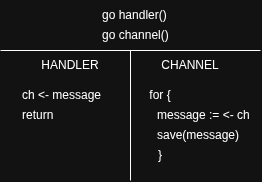
\includegraphics[width=0.6\linewidth]{channelsPseudokod.png}
	\caption{Pseudokód posielania správ}
	\label{channelProgram}
\end{figure}

Vytvoríme groutine pre ukladanie dát, ktorá ukladá správy do databázy. Ďalej vytvoríme goroutine predstavujúcu obsluhu klienta.
Vidíme, že aj pri viacerých klientoch nevznikne problém súbehu a dáta sa zapíšu do databázy správne. Využívame blokovacie
správanie komunikačného kanála, kedy pri prijatí viacerých správ odosielateľ čaká, kým je prijímateľ pripravený spracovať dáta.
Dokážeme si to na príklade dvoch procesov klientov a procesu databázy.
\begin{figure}[htbp]
	\centering
	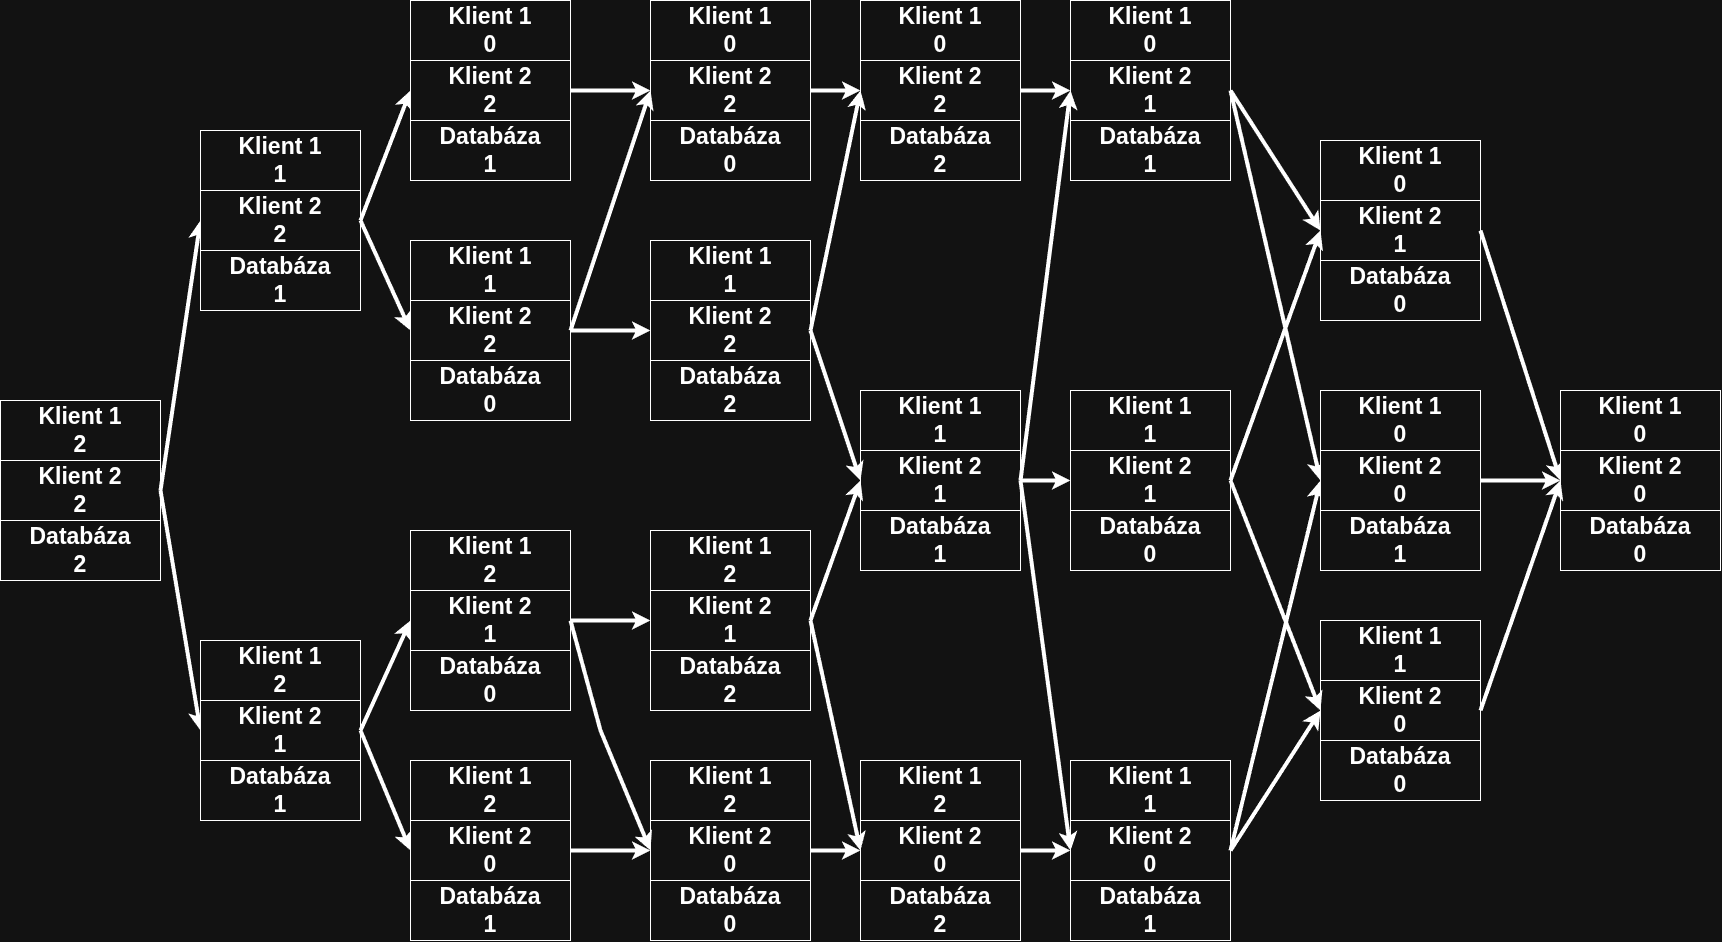
\includegraphics[width=1\linewidth]{channelDokaz.png}
	\caption{Dôkaz posielania správ}
	\label{channelsDokaz}
\end{figure}

Tu vidíme, že procesy klientov sú blokované, kým proces ukladania dát je pripravený prijať dáta. Preto vždy dôjdeme k požadovanému
výsledku.


\appendix
\begin{figure}[htbp]
	\centering
	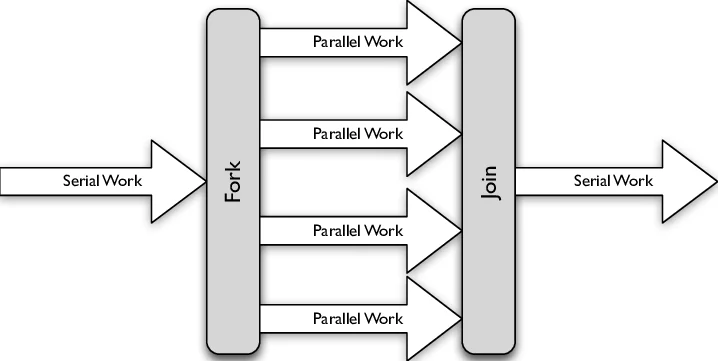
\includegraphics[width=0.6\linewidth]{forkJoinModel.png}
	\caption{Model fork-join}
	\label{fork-join}
\end{figure}
\nocite{*}
\printbibliography


\end{document}
